%%%%%%%%%%%%%%%%%%%%%%%%%%%%%%%%%%%%%%%%%%%%%%%%%%%%%%%%%%%%%%%%%%%%
%% I, the copyright holder of this work, release this work into the
%% public domain. This applies worldwide. In some countries this may
%% not be legally possible; if so: I grant anyone the right to use
%% this work for any purpose, without any conditions, unless such
%% conditions are required by law.
%%%%%%%%%%%%%%%%%%%%%%%%%%%%%%%%%%%%%%%%%%%%%%%%%%%%%%%%%%%%%%%%%%%%

\documentclass[
  digital, %% This option enables the default options for the
           %% digital version of a document. Replace with `printed`
           %% to enable the default options for the printed version
           %% of a document.
  table,   %% Causes the coloring of tables. Replace with `notable`
           %% to restore plain tables.
  lof,     %% Prints the List of Figures. Replace with `nolof` to
           %% hide the List of Figures.
  nolot,     %% Prints the List of Tables. Replace with `nolot` to
           %% hide the List of Tables.
  %% More options are listed in the user guide at
  %% <http://mirrors.ctan.org/macros/latex/contrib/fithesis/guide/mu/fi.pdf>.
]{fithesis3}
%% The following section sets up the locales used in the thesis.
\usepackage[resetfonts]{cmap} %% We need to load the T2A font encoding
\usepackage[T1,T2A]{fontenc}  %% to use the Cyrillic fonts with Russian texts.
\usepackage[
  main=english, %% By using `czech` or `slovak` as the main locale
                %% instead of `english`, you can typeset the thesis
                %% in either Czech or Slovak, respectively.
   czech %% The additional keys allow
]{babel}        %% foreign texts to be typeset as follows:
%%
%%   \begin{otherlanguage}{german}  ... \end{otherlanguage}
%%   \begin{otherlanguage}{russian} ... \end{otherlanguage}
%%   \begin{otherlanguage}{czech}   ... \end{otherlanguage}
%%   \begin{otherlanguage}{slovak}  ... \end{otherlanguage}
%%
%% For non-Latin scripts, it may be necessary to load additional
%% fonts:
\usepackage{paratype}
%%
%% The following section sets up the metadata of the thesis.
\thesissetup{
    date          = 2018/5/21,
    university    = mu,
    faculty       = fi,
    type          = mgr,
    author        = Václav Štěbra,
    gender        = m,
    advisor       = {doc. RNDr. Tomáš Pitner, Ph.D.},
    title         = {Komunikační portál založený na technologii WebRTC},
    TeXtitle      = {Komunikační portál založený na technologii WebRTC},
    keywords      = {online audio communication, onlide video communication, WebRTC, Javascript, HTML5},
    TeXkeywords   = {online audio communication, onlide video communication, WebRTC, Javascript, HTML5},
    abstract      = {The goal of this thesis is to build online meeting portal using the WebRTC technology. The main focus should be placed on scalability in multi-party calls and on great user experience.},
    thanks        = {These are the acknowledgements for my thesis, which can

                     span multiple paragraphs.},
    bib           = example.bib,
}
\usepackage{makeidx}      %% The `makeidx` package contains
\makeindex                %% helper commands for index typesetting.
%% These additional packages are used within the document:
\usepackage{paralist} %% Compact list environments
\usepackage{amsmath}  %% Mathematics
\usepackage{amsthm}
\usepackage{amsfonts}
\usepackage{url}      %% Hyperlinks
\usepackage{markdown} %% Lightweight markup
\usepackage{listings} %% Source code highlighting
\lstset{
  basicstyle      = \ttfamily,%
  identifierstyle = \color{black},%
  keywordstyle    = \color{blue},%
  keywordstyle    = {[2]\color{cyan}},%
  keywordstyle    = {[3]\color{olive}},%
  stringstyle     = \color{teal},%
  commentstyle    = \itshape\color{magenta}}
\usepackage{floatrow} %% Putting captions above tables
\floatsetup[table]{capposition=top}
\begin{document}
\chapter{Introduction}
\section{Motivation}
Online communication is becoming more and more important in today’s world. We use it everyday to communicate with our family, friends and also to communicate with our team members or customers in business environment. Home office or even remote work is becoming more and more popular among many businesses and their employees. With that comes great need for high quality and reliable way of communicating with the rest of the team.

This thesis is a follow up to the bachelor thesis WebRTC meeting portal  \cite{bachelorThesis} written in 2016. It was written as a proof of concept of “relatively” young and not yet widely used technology at that time called WebRTC\footnote{Web Real-Time Communication - https://webrtc.org/
}. Main goal was to build a usable meeting portal using newest web platform capabilities. The main ways of communicating using the portal are audio and video calls between two or more participants. It is also possible to exchange text messages and see the list of participants. Everything is secured so that only invited people can join the meeting.

The meeting portal is very simple and offers many opportunities for new functionality and improvements. It only allows authenticated users to participate in the conference call which on one hand provides better security for the meeting, but on the other hand it can drive some people away as they do not want to create account for yet another service. Especially when they want to use it one time. It was not built with scalability in mind and therefore only very small number of users is able the connect before the quality degrades. There is no possibility to mute the audio or screen share. This thesis elaborates on some of the mentioned shortcomings and also introduces couple new features.

\section{Goal of the thesis}
Main disadvantage of the previous portal are high requirements on the users bandwidth when participating in the multi-party conference call. Therefore biggest focus and architecture goal of this thesis is to build the portal with a higher scalability in mind so that it can handle higher number of participants without big degradation of call quality.

Focus is placed on better user experience. This includes features such as possibility to mute the microphone, disable camera feed or joining  the conference without the user account. Also there will be possibility to share the screen.
 
During the meeting it should be possible to share files between the participants of the call. After the meeting all users with an account who participated in the call will be able to access, view and download the recording of the call.

\section{Structure}
This work is divided into several chapters. First one serves as introduction of the previous work upon which this thesis is built. It sets the goals which this thesis should accomplish.

Second chapter is a brief summary of some of the most popular currently used commercial communication tools with focus on possibility of their use in businesses.

Third chapter is a description of the technologies used to build the portal. It introduces WebRTC in more depth with focus on building scalable communication solutions. It covers backend and frontend technologies, frameworks and libraries used such as Node.js\footnote{https://nodejs.org/en/}, Express\footnote{https://expressjs.com/} and React\footnote{https://reactjs.org/}. It also mentions other tools used during development such as Github\footnote{https://github.com/} and Travis CI\footnote{https://travis-ci.org/}.

Fourth chapter focuses on the requirements for the portal. It states both functional and nonfunctional requirements. It puts most focus on the functionality added to the original portal.

Fifth chapter describes the architecture of the system.

Sixth chapter is concerned with the deployment of the system. It describes how the production server needs to be configured, what needs to be installed on it and how deploy and run the application from the sources.
Seventh chapter is the evaluation of the quality of the meetings made using the implemented solution.

Eight chapter briefly mentions the business potential of the application. It focuses on the minimal requirements / cost of the deployment of the system to the production environment.

Ninth chapter is a summary and evaluation of the accomplished work.

\chapter{Real-time communication applications}

\chapter{Portal Specification}
This chapters summarizes requirements put on the functionality and implementation of the portal.

\section{Functional requirements}
The main use case for the portal is to make group calls between different teams in a business organization. To make these calls as secure as possible there is a choice to restrict the ability to participate in a call to a preselected group of people.

Sometimes there is a also need for communication with outside party, for example with the customers. Because these people are not part of the organization, they have no accounts setup and usually they do not want to be bothered with the process of setting things up. So to make things as easy as possible for them there is a possibility to join the meeting just by accessing the link. 

During the call users can send text messages to all the participants in the shared chat. It is also possible to share files in this chat. Given that just audio and video communication is not enough in some cases there is ability to share the screen. When enabled, all participants of the call can see the screen of the person who initiated the screen sharing. 

After the meeting users can see the history of all the messages sent. The files sent during the meeting are stored on the server so that they can be downloaded after the meeting. The recording of the meeting is also available to download after the meeting has ended. 

All of the use cases are shown in use case diagram in figure~\ref{fig:useCase}

\begin{figure}
  \begin{center}
    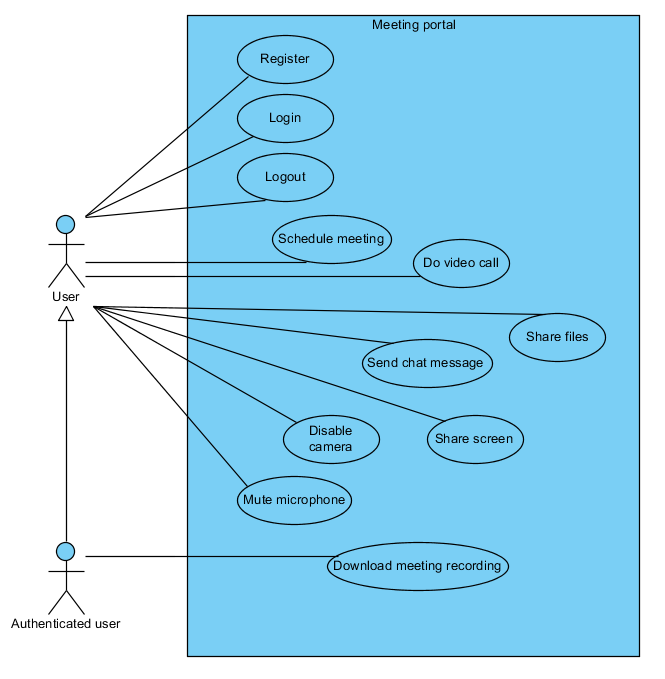
\includegraphics[scale=0.7]{diagrams/use_case.png}
  \end{center}
  \caption{Use case diagram for the portal}
  \label{fig:useCase}
\end{figure}

\section{Nonfunctional requirements}

\chapter{Technologies}

\chapter{Architecture}

\chapter{Deployment}

\chapter{Implementation evaluation}

\chapter{Business evaluation}

\chapter{Conclusion}

\printbibliography[heading=bibintoc] %% Print the bibliography.

\appendix %% Start the appendices.
\chapter{An appendix}
The source code for the portal is available in the archive in the Information System of Masaryk University.

\end{document}
